\chapter[Начало работы]{Начало работы}
\label{chap:getting_started}

\section{Главы и их содержание}

\begin{table}[h]
  \begin{tabulary}{\textwidth}{|L|L|}
    \hline
    Глава & Описание \\
    \hline
    1. Обзор & Описание прибора \\
    \hline
    2. Начало работы & Знакомство с руководством и описание составных частей
    прибора \\
    \hline
    3. Подготовка к работе & Подготовка вашего прибора CG-6
    Autograv\texttrademark{} к проведению съёмки \\
    \hline
    4. Эксплуатация & Эксплуатация прибора \cg{} при
    проведении съёмки \\
    \hline
    5. Техническое обслуживание & Как проводить техническое обслуживание и
    устранять неполадки в приборе \cg{} \\
    \hline
    6. Справочная информация & Технические характеристики, спецификация деталей
    прибора, и сведения о гарантии \\
    \hline
  \end{tabulary}
\end{table}

\section{Условные обозначения}

\warningbox{
  Содержится указание на важный предмет обсуждения, этому разделу нужно уделить
  особое внимание
}

\infobox{
  Акцентируется внимание на информации, представляющей особый интерес для
  пользователя
}

Необходимые для выполнения действия, такие как <<нажать>>, <<ввести>> и
<<редактировать>>, выделяются \textit{курсивом}. Кнопки клавиатуры выделяются
\textbf{жирным шрифтом}. Пункты меню выделяются заглавными буквами и
\textbf{ЖИРНЫМ ШРИФТОМ}.

\section{Распаковка прибора}

Прибор \cg{} упакован в кофр с мягкими вставками (при
этом, аккумуляторные батареи располагаются отдельно, в индивидуальной упаковке,
в соответствии с правилами безопасности на транспорте IATA), которые
обеспечивают защиту прибора во время доставки и перевозки.

\warningbox{
  Перевозка прибора должна осуществляться с извлечёнными аккумуляторными
  батареями. Батареи должны размещаться отдельно. Если вы только что получили
  прибор \cg{}, имейте в виду, что аккумуляторные
  батареи упакованы отдельно, и заряжены примерно на 30\% от номинального
  объёма.
}

\begin{figure}%[]
  \centering
  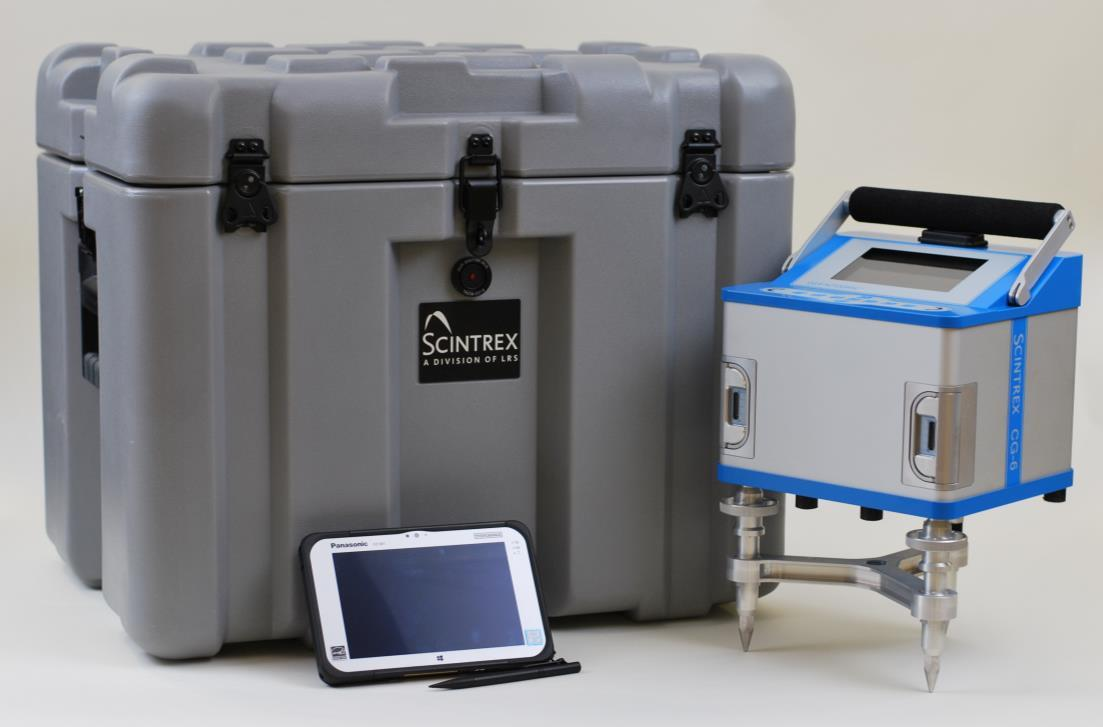
\includegraphics[width=\textwidth]{figures/the_cg6_autograv_gravity_meter_and_its_transportation_case}
  \caption{Гравиметр \cg{} и транспортировочный ящик}
  \label{fig:the_cg6_autograv_gravity_meter_and_its_transportation_case}
\end{figure}

\begin{enumerate}
  \item Надавите на красный клапан сброса избыточного давления, расположенный на
    передней стороне транспортировочного кофра.

  \item\label{item:turn_back} Откиньте вверх язычок фиксатора и поверните язычок против часовой
    стрелки, чтобы фиксатор отсоединился от запорной планки.

  \item Повторите действия по п.~\ref{item:turn_back} для других фиксаторов.

  \begin{figure}[h]
    \centering
    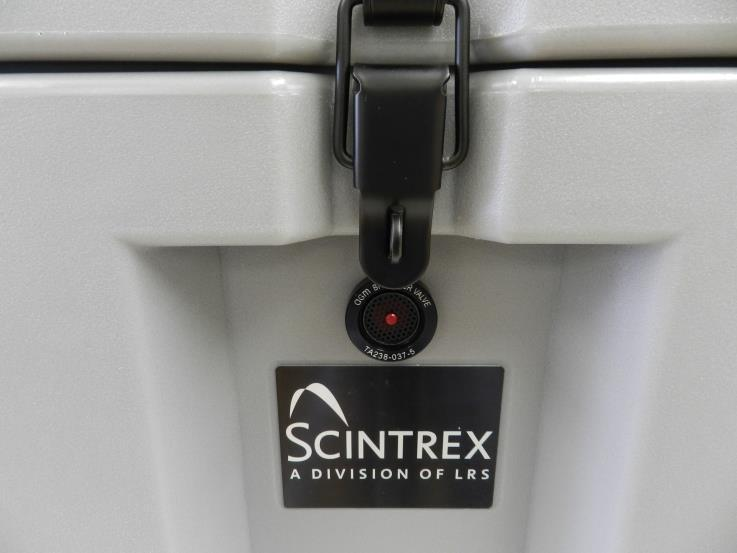
\includegraphics[width=0.7\textwidth]{figures/location_of_the_pressure_release_value_on_the_transportation_case}
    \caption{Клапан сброса избыточного давления на кофре}
    \label{fig:location_of_the_pressure_release_value_on_the_transportation_case}
  \end{figure}

  \item Откройте транспортировочный кофр прибора CG-6
    Autograv\texttrademark{}, подняв крышку.

  \item Извлеките прибор \cg{} из транспортировочного
    кофра, потянув его вертикально вверх за чёрную резиновую ручку. Произведите
    визуальный осмотр прибора на наличие физических повреждений, которые могут
    быть получены во время транспортировки.
\end{enumerate}

\warningbox{
  Транспортировочный кофр прибора CG-6 Autograv\texttrademark{} снабжён
  индикатором удара Shockwatch, который закреплён на боковой стенке.  Проверьте
  индикатор, и если вы обнаружите, что контрольный элемент окрашен в красный
  цвет, немедленно обратитесь в компанию Scintrex Limited.  Обратитесь к разделу
  \nameref{sec:shipping_instructions} на
  странице~\pageref{sec:shipping_instructions}.
}

\begin{figure}%[]
  \centering
  
\includegraphics[width=0.7\textwidth]{figures/shockwatch_monitor}
  \caption{Индикатор удара Shockwatch}
  \label{fig:shockwatch_monitor}
\end{figure}

\section{Обзор составных частей}

На следующем рисунке показан вид сверху всех компонентов, которые поставляются
со стандартной комплектацией \cg{} в транспортировочном
кейсе.

\begin{figure}%[]
  \centering
  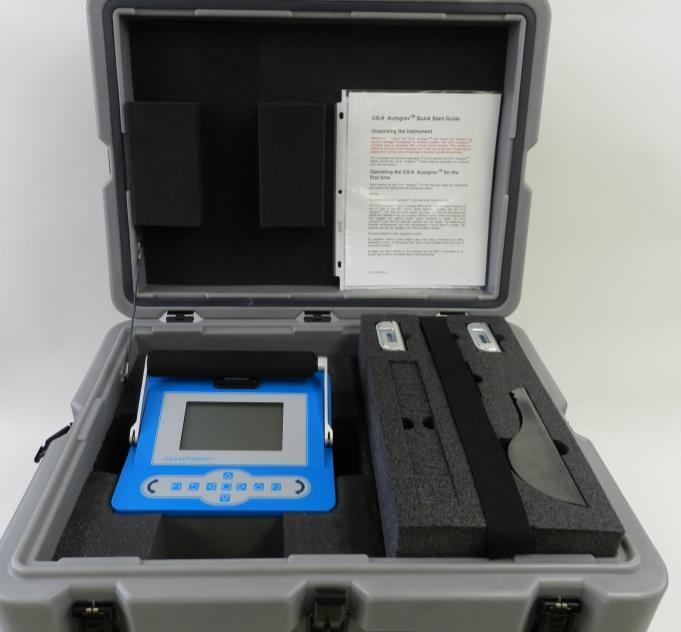
\includegraphics[width=0.7\textwidth]{figures/the_cg6_autograv_and_its_components}
  \caption{Прибор \cg{} и его составные части}
  \label{fig:the_cg6_autograv_and_its_components}
\end{figure}

\section{Обзор панели управления и клавиатуры}

На рисунке~\ref{fig:the_cg6_autograv_console} изображена передняя панель
прибора. Она состоит из дисплея, антенны GPS/Bluetooth, модуля клавиатуры, для
управления прибором и светодиодных стрелок для нивелирования.

\begin{figure}%[]
  \centering
  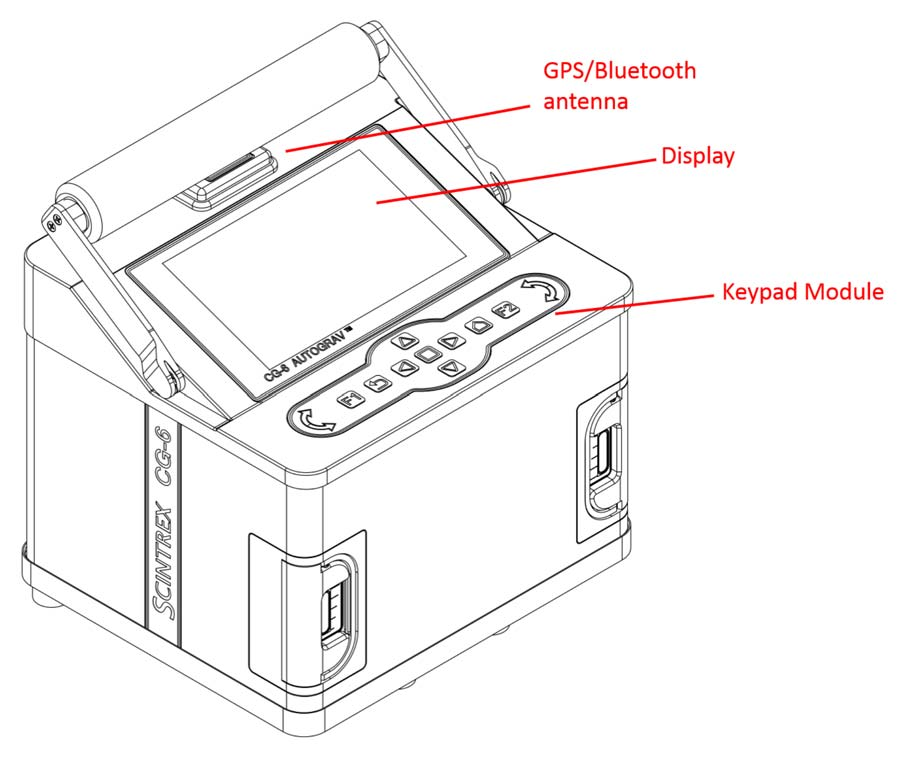
\includegraphics[width=0.7\textwidth]{figures/the_cg6_autograv_console}
  \caption{Панель управления прибора \cg{}}
  \label{fig:the_cg6_autograv_console}
\end{figure}

\begin{figure}%[]
  \centering
  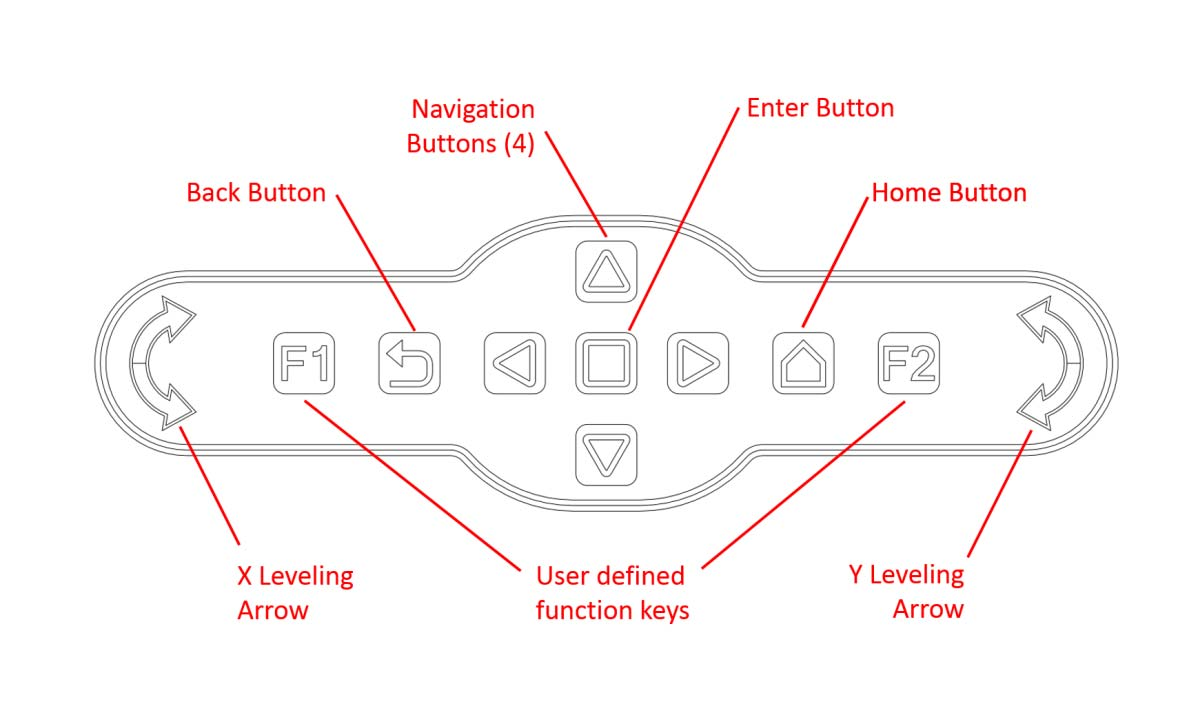
\includegraphics[width=0.7\textwidth]{figures/the_cg6_autograv_keypad_module}
  \caption{Модуль клавиатуры CG-6 Autograv}
  \label{fig:the_cg6_autograv_keypad_module}
\end{figure}

Две стрелки указывают направление, в котором нужно вращать нивелировочные винты
для выравнивания треноги. Стрелка слева относится к левому нивелировочному
винту, а стрелка справа~-- к правому нивелировочному винту.  Правый винт
выравнивает прибор одновременно по осям X и Y, тогда как левый винт выравнивает
прибор только по оси X.

\infobox{
  Хотя для грубого выравнивания можно вращать оба винта штатива одновременно,
  для точного выравнивания может оказаться более эффективным сначала правым
  винтом отрегулировать уровень по оси Y, после этого левым винтом
  отрегулировать уровень по оси X.
}

Вы можете перемещаться между элементами меню, расположенными в нижней части
экрана, используя \textbf{кнопки Navigation} <<Навигация>>, \textbf{Home} <<На
главный экран>>, \textbf{Back} <<Назад>>, \textbf{F1} и \textbf{F2}. На любом
экране переместите курсор либо на \textbf{BACK}, либо на \textbf{CANCEL} и
нажмите кнопку \textbf{Enter}, либо нажмите кнопку \textbf{Back}, чтобы
вернуться к предыдущему экрану. Нажмите кнопку Home, чтобы перейти на главный
экран.

\section[Ввод в работу]{Ввод в работу прибора \cg{}}

Если прибор \cg{} включается в первый раз, или если он
был выключен более 24 часов, необходимо выполнить следующие действия, соблюдая
определённые периоды ожидания.

\paragraph[Подача питания]{Подача питания на прибор \cg{}:} обратитесь к расположенному ниже
разделу под заголовком: \nameref{subsec:powering_up_the_cg6_autograv}

\paragraph{Период прогревания:} после подачи питания на прибор \cg{}{}, время,
необходимое для достижения рабочей температуры, составляет примерно один час.

\paragraph{Период стабилизации:} после подачи питания на прибор требуется 24
часа на его стабилизацию.

\paragraph{Подготовка прибора для полевых работ:} по завершении периода
стабилизации, ваш прибор \cg{} готов к работе.
Обратитесь к следующей главе (Настройка \cg{}), где
содержится подробная информация о подготовке прибора к работе.

\subsection[Подача питания]{Подача питания на прибор \cg{}}
\label{subsec:powering_up_the_cg6_autograv}

Подачу питания на прибор \cg{} можно осуществлять одним
из следующих способов:
\begin{itemize}
  \item От внешнего источника постоянного тока напряжением 15В.

    \begin{figure}[h]
      \centering
      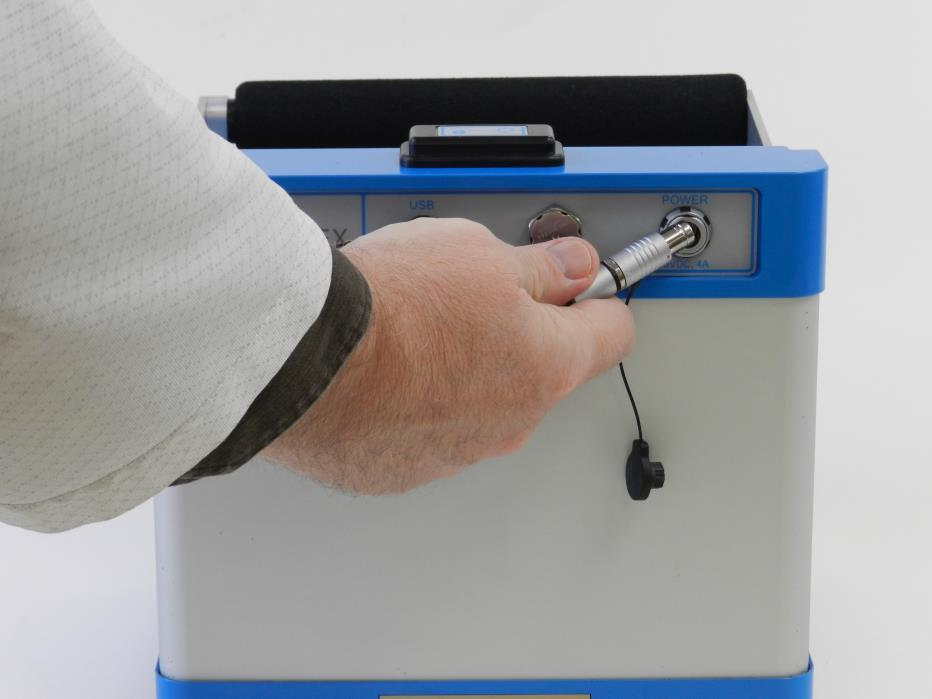
\includegraphics[width=0.7\textwidth]{figures/connecting_the_power_supply_to_the_cg6_autograv}
      \caption{Подключение внешнего источника питания к \cg{}}
      \label{fig:connecting_the_power_supply_to_the_cg6_autograv}
    \end{figure}

  \item От двух встроенных интеллектуальных аккумуляторных батарей, которые
    поставляются вместе с прибором \cg{}.

    \begin{figure}[h]
      \centering
      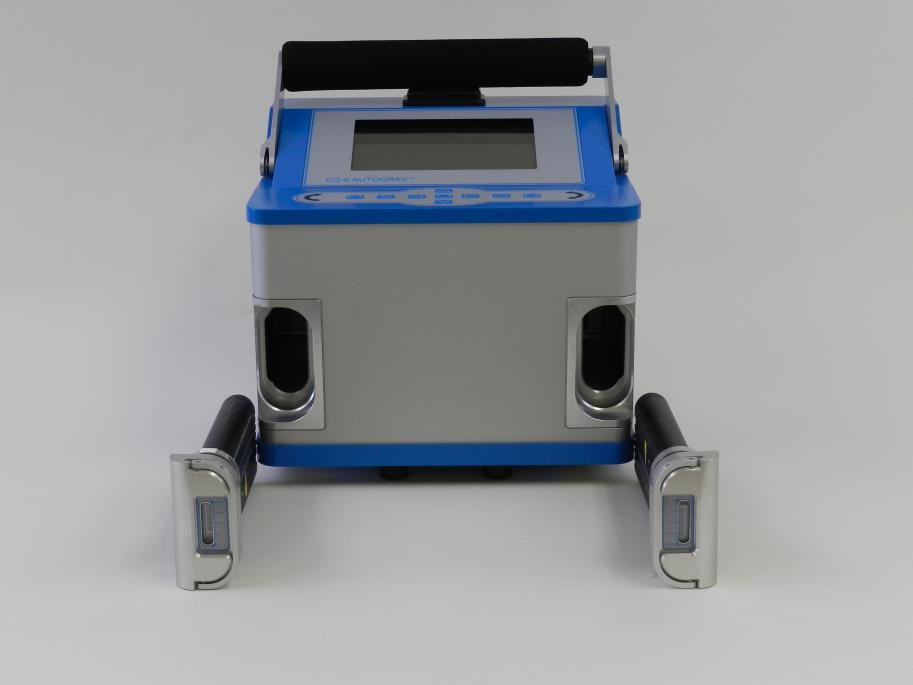
\includegraphics[width=0.7\textwidth]{figures/the_cg6_autograv_and_batteries}
      \caption{Прибор \cg{} с аккумуляторными батареями}
      \label{fig:the_cg6_autograv_and_batteries}
    \end{figure}
\end{itemize}

Если при подключении внешнего источника питания аккумуляторные батареи уже
находятся в рабочем положении, источник питания будет обеспечивать прибор
электроэнергией, а в случае необходимости будет также заряжать аккумуляторные
батареи. После полной зарядки аккумуляторных батарей источник питания будет
продолжать подачу электроэнергии на прибор, поддерживая аккумуляторные батареи в
полностью заряженном состоянии. На зарядку полностью разряженных батарей уходит
приблизительно 4 часа. Зарядка обеих батарей происходит одновременно.

\infobox{
  Когда питание прибора \cg{} осуществляется от двух батарей, они
  разряжаются с одинаковой скоростью.
}

\subsection[Зарядка аккумуляторных батарей]{Зарядка аккумуляторных батарей прибора \cg{}}

Помимо возможности производить зарядку батарей в полевых условиях
непосредственно в приборе CG-6 AutogravTM, батареи можно заряжать с помощью
зарядного устройства с микропроцессорным управлением (\textnumero{}~400209):

\begin{figure}[h]
  \centering
  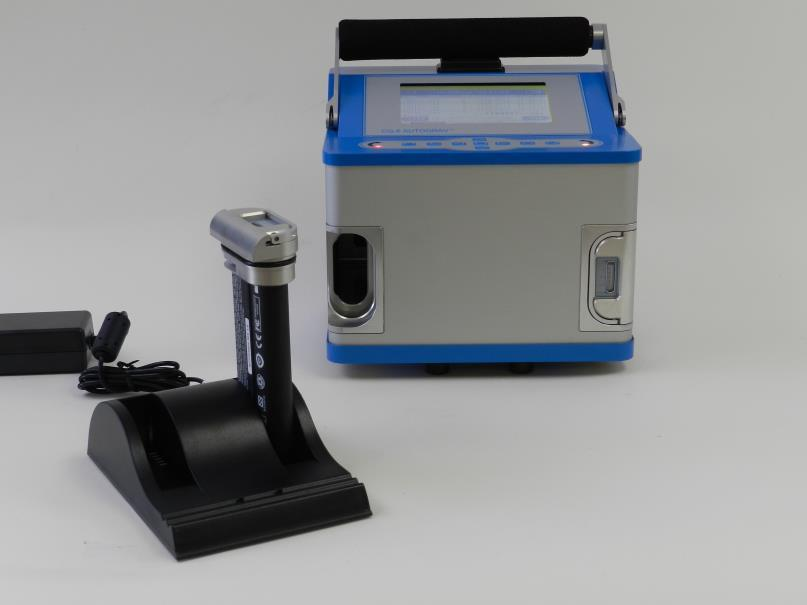
\includegraphics[width=0.7\textwidth]{figures/the_cg6_autograv_gravity_meter_and_the_battery_charger}
  \caption{\cg{} и устройство зарядки аккумуляторных батарей}
  \label{fig:the_cg6_autograv_gravity_meter_and_the_battery_charger}
\end{figure}

\section{Обзор главного экрана изображения}

\begin{figure}[h]
  \centering
  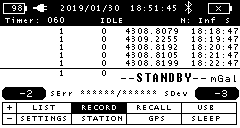
\includegraphics[width=0.49\textwidth]{figures/cg6_autograv_main_screen_idle_mode}
  \caption{Главный экран \cg{}: режим ожидания}
  \label{fig:cg6_autograv_main_screen_idle_mode}
\end{figure}

\begin{figure}[h]
  \centering
  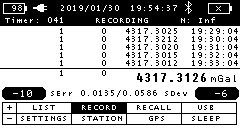
\includegraphics[width=0.49\textwidth]{figures/cg6_autograv_main_screen_recording_mode}
  \caption{Главный экран \cg{}: режим записи}
  \label{fig:cg6_autograv_main_screen_recording_mode}
\end{figure}

В верхней части главного экрана находятся; значки статуса батарей (с указанием
процента заряда каждой аккумуляторной батареи). Дата и время, показания таймера
(оставшееся время измерения текущего цикла в секундах, обратный отсчёт времени
регистрации), статус измерительного прибора (находится ли он в режиме
бездействия (IDLE) или в режиме регистрации данных (RECORDING)) и число циклов,
запрограммированное для проведения измерений.

\begin{figure}[h]
  \centering
  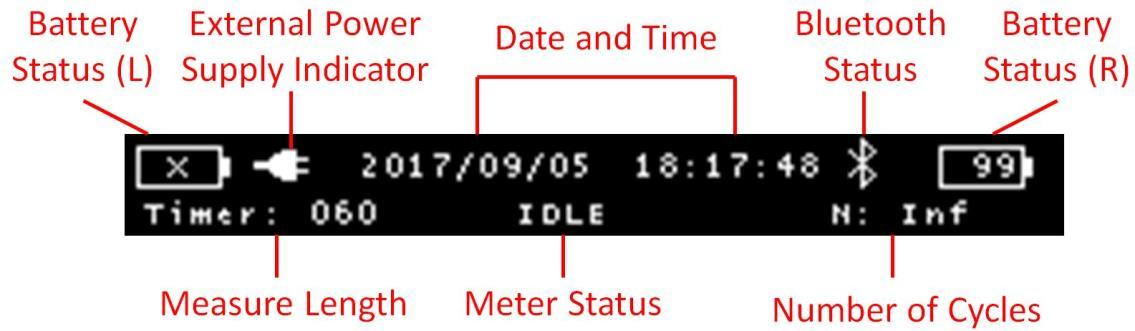
\includegraphics[width=0.7\textwidth]{figures/main_screen_upper_part}
  \caption{Главный экран: верхняя часть}
  \label{fig:main_screen_upper_part}
\end{figure}

В средней части экранного изображения отображаются предыдущие измерения силы
тяжести, где наиболее удалённые по времени измерения располагаются вверху
списка. Здесь отображаются также название пункта наблюдения, номер профиля,
величина измерения и время в конце взятия отсчётов. Эти измерения уже сохранены
в памяти прибора.

\begin{figure}[h]
  \centering
  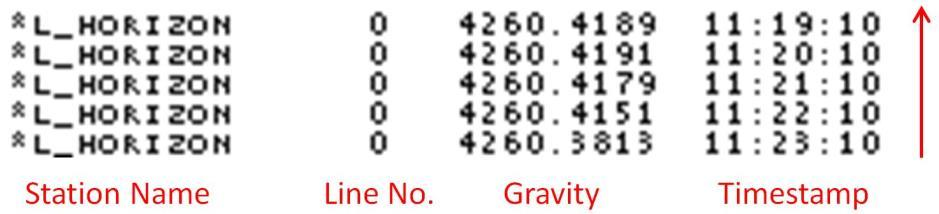
\includegraphics[width=0.7\textwidth]{figures/main_screen_middle_part}
  \caption{Главный экран: средняя часть}
  \label{fig:main_screen_middle_part}
\end{figure}

Под сплошной горизонтальной линией отображается: текущий пункт наблюдения и его
порядковый номер в списке пунктов наблюдения, номер профиля. А под ними –
величина измерения в мГал, величина стандартного отклонения (SDev) для отсчётов,
использованных для расчёта измерения, и величина стандартной ошибки (SErr,
равной стандартному отклонению, разделённому на квадратный корень из числа
текущих отсчётов $ SErr = SDev/\sqrt{N} $). Когда измеритель находится в режиме
ожидания, значение силы тяжести заменяется на <<STANDBY>> и значения SErr и SDev
будут *****

Слева показана величина наклона по оси X в арксекундах, а справа – величина
наклона по оси Y в арксекундах.

\begin{figure}[h]
  \centering
  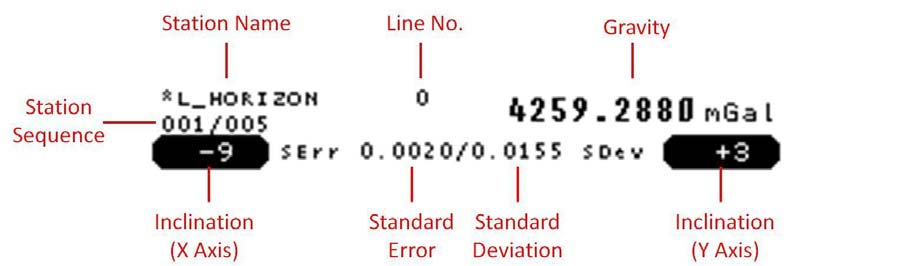
\includegraphics[width=0.7\textwidth]{figures/main_screen_lower_part}
  \caption{Главный экран: нижняя часть}
  \label{fig:main_screen_lower_part}
\end{figure}

В нижней части экрана располагаются наиболее часто используемые элементы меню.

\begin{figure}[h]
  \centering
  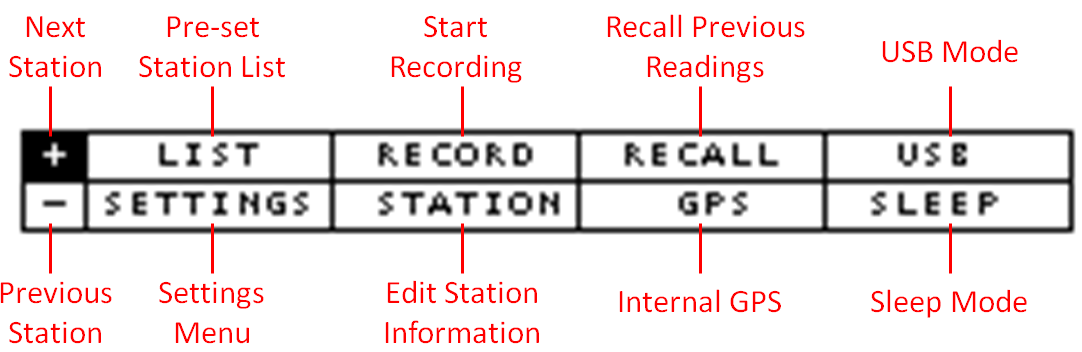
\includegraphics[width=0.7\textwidth]{figures/main_screen_menu}
  \caption{Меню главного экрана}
  \label{fig:main_screen_menu}
\end{figure}

\section{Базовые операции}

\subsection{Перемещение по меню}

При помощи кнопок управления осуществляется перемещение курсора.  Подтверждение
выбора или вход в подменю производится с помощью кнопки \textbf{Enter}.

\begin{figure}[h]
  \centering
  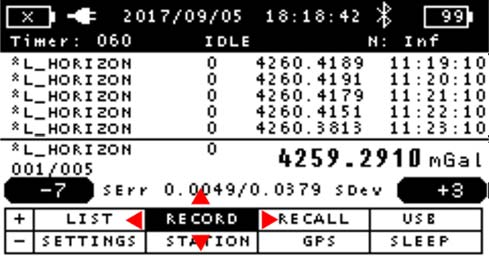
\includegraphics[width=0.49\textwidth]{figures/navigation_the_menus_1}
  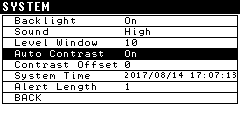
\includegraphics[width=0.49\textwidth]{figures/navigation_the_menus_2}
  \caption{Перемещение по меню}
  \label{fig:navigation_the_menus}
\end{figure}

\subsection{Снятие показаний}

Счётчик имеет два режима работы:
\begin{description}
  \item[RECORDING (ЗАПИСЬ):] Используется для записи измерений. В этом режиме
    отфильтрованное значение силы тяжести отображается на главном экране, как
    показано на рисунке~\ref{fig:cg6_autograv_main_screen_recording_mode}.

  \item[IDLE (ХОЛОСТОЙ ХОД):] Используется при перемещении прибора. Это
    сокращает время установки на следующей станции за счёт стабилизации
    электроники во время транспортировки. В этом режиме значение силы тяжести
    заменяется словом “STANDBY” на главном экране, как показано на
    рисунке~\ref{fig:cg6_autograv_main_screen_idle_mode}. 
\end{description}

Для переключения режима работы между \textit{\textbf{RECORDING}} и
\textit{\textbf{IDLE}}: поместите курсор на \textbf{RECORD} на главном экране и
нажмите кнопку \textbf{Enter}.

\subsection{Редактирование значений переменных}

\subsubsection{Как выделить значение в выбираемом списке}

\begin{figure}[h]
  \centering
  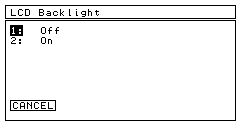
\includegraphics[width=0.49\textwidth]{figures/choosing_a_value_from_a_selectable_list}
  \caption{Выделение значения в выбираемом списке}
  \label{fig:choosing_a_value_from_a_selectable_list}
\end{figure}

Для того, чтобы выделить значение в выбираемом списке, достаточно навести курсор
на нужную запись и нажать кнопку \textbf{Enter}.

Чтобы покинуть это экранное изображение без изменений:
\begin{itemize}
  \item наведите курсор на пункт \textbf{CANCEL}, после чего нажмите кнопку
    \textbf{Enter}, или
  \item нажмите кнопку \textbf{Back}
\end{itemize}

\subsubsection{Ввод значения с экранной клавиатуры}
\label{subsubsec:entering_a_value_with_onscreen_keypad}

Некоторые переменные требуют редактирования с помощью экранной клавиатуры.  В
зависимости от типа переменной, экранная клавиатура может быть цифровой или
буквенно-цифровой.

\begin{figure}[h]
  \centering
  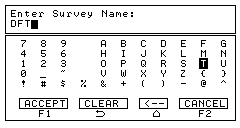
\includegraphics[width=0.49\textwidth]{figures/onscreen_keypad_numeric_and_alphanumeric_1}
  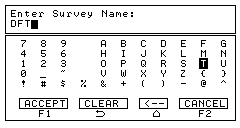
\includegraphics[width=0.49\textwidth]{figures/onscreen_keypad_numeric_and_alphanumeric_2}
  \caption{Экранная клавиатура: цифровая и буквенно-цифровая}
  \label{fig:onscreen_keypad_numeric_and_alphanumeric}
\end{figure}

Чтобы ввести символ в поле, переместите курсор на нужный символ и нажмите кнопку
\textbf{Enter}.

Чтобы стереть последний символ в поле, переместите курсор на $\leftarrow$ , используя:
\begin{itemize}
  \item кнопки навигации \textbf{Navigation}, или
  \item кнопку \textbf{Home}
\end{itemize}
и нажмите кнопку \textbf{Enter}.

Чтобы очистить все поле, переместите курсор на \textbf{<<CLEAR>>} используя:
\begin{itemize}
  \item кнопки навигации \textbf{Navigation}, или
  \item кнопку \textbf{Back}
\end{itemize}
и нажмите кнопку \textbf{Enter}.

Чтобы принять значение в поле, переместите курсор на \textbf{<<ACCEPT>>} используя:
\begin{itemize}
  \item кнопки навигации \textbf{Navigation}, или
  \item кнопку \textbf{F1}
\end{itemize}
и нажмите кнопку \textbf{Enter}.

Чтобы выйти из этого экрана без изменений, переместите курсор на
\textbf{<<CANCEL>>}, используя:
\begin{itemize}
  \item кнопки навигации \textbf{Navigation}, или
  \item кнопку \textbf{F2}
\end{itemize}
и нажмите кнопку \textbf{Enter}.

\section[Спящий режим]{Ввод/вывод прибора \cg{} в/из спящего режима}

Прибор \cg{} может быть переведён в спящий режим, когда бездействует главный
дисплей и стрелки выравнивания. Однако, сам прибор остаётся в рабочем состоянии.

\begin{figure}[h]
  \centering
  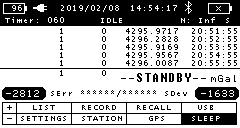
\includegraphics[width=0.49\textwidth]{figures/the_main_screen_ready_for_sleep_mode}
  \caption{Главный экран готов к спящему режиму}
  \label{fig:the_main_screen_ready_for_sleep_mode}
\end{figure}

На главном экранном изображении при помощи \textbf{кнопок управления Navigation}
наведите курсор на пункт \textbf{SLEEP} и нажмите кнопку \textbf{Enter}.

\infobox{
  Когда прибор \cg{} находится в спящем режиме, нажатие любой кнопки приведёт к
  его <<пробуждению>>.
}
